\documentclass[onecolumn, draftclsnofoot,10pt, compsoc]{IEEEtran}
\usepackage{graphicx}
\usepackage{url}
\usepackage{setspace}
\usepackage{listings}
\usepackage{color}
\usepackage{geometry}
\usepackage{float}
\geometry{textheight=9.5in, textwidth=7in}

\definecolor{mygreen}{rgb}{0,0.6,0}
\definecolor{mygray}{rgb}{0.5,0.5,0.5}
\definecolor{mymauve}{rgb}{0.58,0,0.82}

\lstset{
	backgroundcolor=\color{white},
	basicstyle=\footnotesize,
	captionpos=b,
	frame=single,
	keywordstyle=\color{blue},
	language=HTML,
	numbers=left,
	numberstyle=\tiny\color{mygray},
	tabsize=2
}
	
	

% 1. Fill in these details
\def \CapstoneTeamName{		Stat Champs}
\def \CapstoneTeamNumber{		59}
\def \GroupMemberOne{			Alex Hoffer}
\def \GroupMemberTwo{			Chongxian Chen}
\def \GroupMemberThree{			Jacob Smith}
\def \CapstoneProjectName{		Machine Learn Your Way to March Madness Glory}
\def \CapstoneSponsorCompany{	Oregon State University}
\def \CapstoneSponsorPerson{		Dr. Victor Hsu}

% 2. Uncomment the appropriate line below so that the document type works
\def \DocType{		%Problem Statement
				%Requirements Document
				%Technology Review
				Progress Report
				}
			
\newcommand{\NameSigPair}[1]{\par
\makebox[2.75in][r]{#1} \hfil 	\makebox[3.25in]{\makebox[2.25in]{\hrulefill} \hfill		\makebox[.75in]{\hrulefill}}
\par\vspace{-12pt} \textit{\tiny\noindent
\makebox[2.75in]{} \hfil		\makebox[3.25in]{\makebox[2.25in][r]{Signature} \hfill	\makebox[.75in][r]{Date}}}}
% 3. If the document is not to be signed, uncomment the RENEWcommand below
\renewcommand{\NameSigPair}[1]{#1}

%%%%%%%%%%%%%%%%%%%%%%%%%%%%%%%%%%%%%%%
\begin{document}
\pagenumbering{arabic}
\begin{centering}
\huge
Spring Term Progress Report \\
\Large 
\textbf{Name:} Alex Hoffer, Chongxian Chen, Jacob Smith \\
\textbf{Group Number:} 59 \\
\textbf{Project Title:} Machine Learn Your Way to March Madness Glory! \\
\end{centering}
%\begin{titlepage}
%\pagenumbering{gobble}
 \begin{singlespace}
   % 	\includegraphics[height=4cm]{coe_v_spot1}
    %    \hfill 
        % 4. If you have a logo, use this includegraphics command to put it on the coversheet.
        %\includegraphics[height=4cm]{CompanyLogo}   
     %   \par\vspace{.2in}
      %  \centering
 %       \scshape{
  %          \huge CS Capstone \DocType \par
   %         {\large\today}\par
    %        \vspace{.5in}
     %       \textbf{\Huge\CapstoneProjectName}\par
      %      \vfill
       %     {\large Prepared for}\par
        %    \Huge \CapstoneSponsorCompany\par
         %   \vspace{5pt}
          %  {\Large\NameSigPair{\CapstoneSponsorPerson}\par}
           % {\large Prepared by }\par
           % Group\CapstoneTeamNumber\par
            % 5. comment out the line below this one if you do not wish to name your team
         %   \CapstoneTeamName\par 
        %    \vspace{5pt}
       %     {\Large
      %          \NameSigPair{\GroupMemberOne}\par
     %           \NameSigPair{\GroupMemberTwo}\par
    %            \NameSigPair{\GroupMemberThree}\par
          %  }
   %         \vspace{20pt}
  %      }
      	 \begin{abstract}
        % 6. Fill in your abstract    
        %	This document is written using one sentence per line.
        %	This allows you to have sensible diffs when you use \LaTeX with version control, as well as giving a quick visual test to see if sentences are too short/long.
        %	If you have questions, ``The Not So Short Guide to LaTeX'' is a great resource (\url{https://tobi.oetiker.ch/lshort/lshort.pdf})
	The application of machine learning to Biochemistry and Biophysics has enabled researchers in this field to make remarkable discoveries, such as the generation of new DNA sequences. However, students of Biochemistry and Biophysics do not get the opportunity to learn machine learning. Dr. Victor Hsu of the Oregon State University Biochemistry and Biophysics department has commissioned the Stat Champs to produce an instructional module to give his students the chance to familiarize themselves with machine learning. The software product the Stats Champs have agreed to develop is a web page that allows students to train a machine learning model based on the college basketball statistics and machine learning algorithm of their choosing in order to produce a March Madness bracket. This will help students understand how machine learning algorithms produce models and how inclusion or exclusion of certain data can influence such models. Over the course of Fall term 2016, the Stat Champs developed materials such as design documents and technology reviews in order to prepare for the engineering of the module. Then, in Winter term 2017, the Stat Champs began the software development phase of this project. In Spring term 2017, the project was finished. This report comprehensively describes the process of finishing up the project.
      	\end{abstract}     
 	\end{singlespace}
	%\end{titlepage}
\newpage
%\pagenumbering{arabic}
\tableofcontents
% 7. uncomment this (if applicable). Consider adding a page break.
%\listoffigures
%\listoftables
\clearpage

% 8. now you write!
\section{Introduction}
Biochemistry and Biophysics are two fields that are ripe with many exciting breakthroughs. Machine learning is used by these disciplines to aid their research by providing the ability to generate new sequences of DNA. Our client, Dr. Victor Hsu, is a professor in the Biochemistry and Biophysics department at OSU who recognized that his students should understand machine learning in order to prepare them for their careers. He noticed that the department does not encourage learning machine learning, and that even if they were to, machine learning is a difficult topic for people who haven't been trained in computer science. Additionally, learning machine learning through its application to these fields can be confusing, since machine learned models of DNA can be tough to interpret. Therefore, he commissioned us to produce an online instructional module where his students could grasp machine learning fundamentals in a fun and straightforward manner. To achieve this, he asked us to provide an interface where users could select from men's college basketball statistics and generate a March Madness bracket. In doing so, budding scientists would be able to familiarize themselves with basic machine learning algorithms and also witness how the inclusion or exclusion of data influences the models trained on them. This report chronicles the progress of our team through our final term.

\section{Alex}

\subsection{Where Alex is At On the Project}
Alex completed his requirements early in the winter term. Thus, the only things he can do now are to make the module look nicer, though any changes made now won't be included in the product version that we will be presenting at Expo on May 19, because it would run the risk of introducing bugs. Since our current module satisfies all functional requirements, it would be unwise to add code that could meddle with its performance. It may be nice to format the bracket that is generated in a way that is more appealing, colorful, and relevant. Perhaps this could mean adding a cool March Madness logo somewhere. If we were to polish the module more, while it would not add any \emph{pizzazz} to the Expo version, it would make our project more marketable to potential employers.

\subsection{What Alex Has Left To Do}
The remaining parts of this class that Alex has left to do are: present at Expo, turn in the spring term progress report, and complete the writing assignments needed at the end. There are no remaining things for Alex to do on the project in terms of \emph{required functionality}. Everything that was asked by our client has been completed. If he wants to, he can polish the bracket output to make it look more presentable. Currently, it does look a bit boring, which is unfortunate for a module that does something so interesting.

\subsection{Problems that have impeded my progress}
I am reasonably well acquainted with web development and so my responsibilities did not pose me much grief. However, my JavaScript ability is somewhat lacking. So, I would say that the real problems I ran into in fulfilling my tasks were my neophytic JavaScript skills. One concrete issue that I ran into that I still need to resolve is how the web page appears on different browsers. The computer I used to do my development runs on Windows and I use a Chrome browser. But, when my partner pulled up the web page on a computer running an Apple operating system in a Safari browser, the divisions between the subpages of the site became unset and looked disorganized. This could be a problem because many people use Apple computers and I don't want my hard work in a high quality user experience to go to waste just because of a lack of empathy for running software on different platforms. I also noticed that even on my browser there remains a few spots where the organization is slightly off, for example, on my group description page the text occupies too much space and is to close to the button on the bottom. I want to make this text smaller so that it does not crowd the user's vision and distract from proper navigation through the module. Additionally, I used to have a banner across the top that allowed users to select which part of the project they wanted to visit, but I changed it to a small menu button that provides this service instead. I aim to change it back. Sadly, I will have to make these changes to the product that won't be shown at Expo. In terms of the whole project, we did run into some issues with the machine learning module, particularly the fact that the embedded Python necessary to generate brackets didn't work on the OSU server. Chongxian solved this problem by switching us over to Amazon Web Services (AWS). One more intangible issue we ran into over the course of the whole project was that it was unclear when different parts of the project should be done. A lot of parts of the project depended on other parts, so it was impossible to complete them without completing the others. Since the project is finished, there's no way to change that now, but in future projects, it would be nice to run on a more rigidly defined schedule.

\subsection{Particularly interesting pieces of code}
\begin{lstlisting}[caption=HTML code that uses an icon class to load an envelope icon that links to my email, label=list1]
<div class="col-lg-4 text-center">
	<i class="fa fa-envelope-o fa-3x sr-contact"></i>
	<p><a href="mailto:hoffera@oregonstate.edu">Contact Alex Hoffer</a></p>
</div>
\end{lstlisting}

\subsection{Images from my parts of the project}
A more in-depth description of the images I'll be including:

\begin{enumerate}
\item A home page, found in \textit{Fig. 1}. It includes a a bold title of our project, a photo of an OSU basketball player driving on a UCLA player, a button that changes color when you hover over it, and a menu that upon a click drops down to reveal links to the remaining sections of the page.
\item An instructions page, found in \textit{Fig. 2}, that includes instructions on how to use the module.
\item A module page, located in \textit{Fig. 3}, where the machine learning module hosted on AWS is linked to. Naturally, we were going to host it on this page itself (on OSU's server), but the server didn't support what we wanted to do.
\item A purpose page, represented by \textit{Fig. 4}, where I wrote a short description of why the project was made. Underneath this text lies a button which takes the user to the next section, where I describe our development team and our project information. As described in the "Past Problems" subsection, I need to scrunch up this text to make it all appear without making the page a little disorganized. 
\item An About the Authors page, found in \textit{Fig. 5}. Here I include information about us and a cool email shaped button with the text "Contact Alex Hoffer" underneath it. If the email shaped button is pressed, it executes the script "mailto:hoffera@oregonstate.edu", which is my email. In my "Particularly interesting pieces of code" section, I have included the recipe for invoking this cool button in HTML.
\end{enumerate}  
\newpage

\begin{figure}[H]
\centering
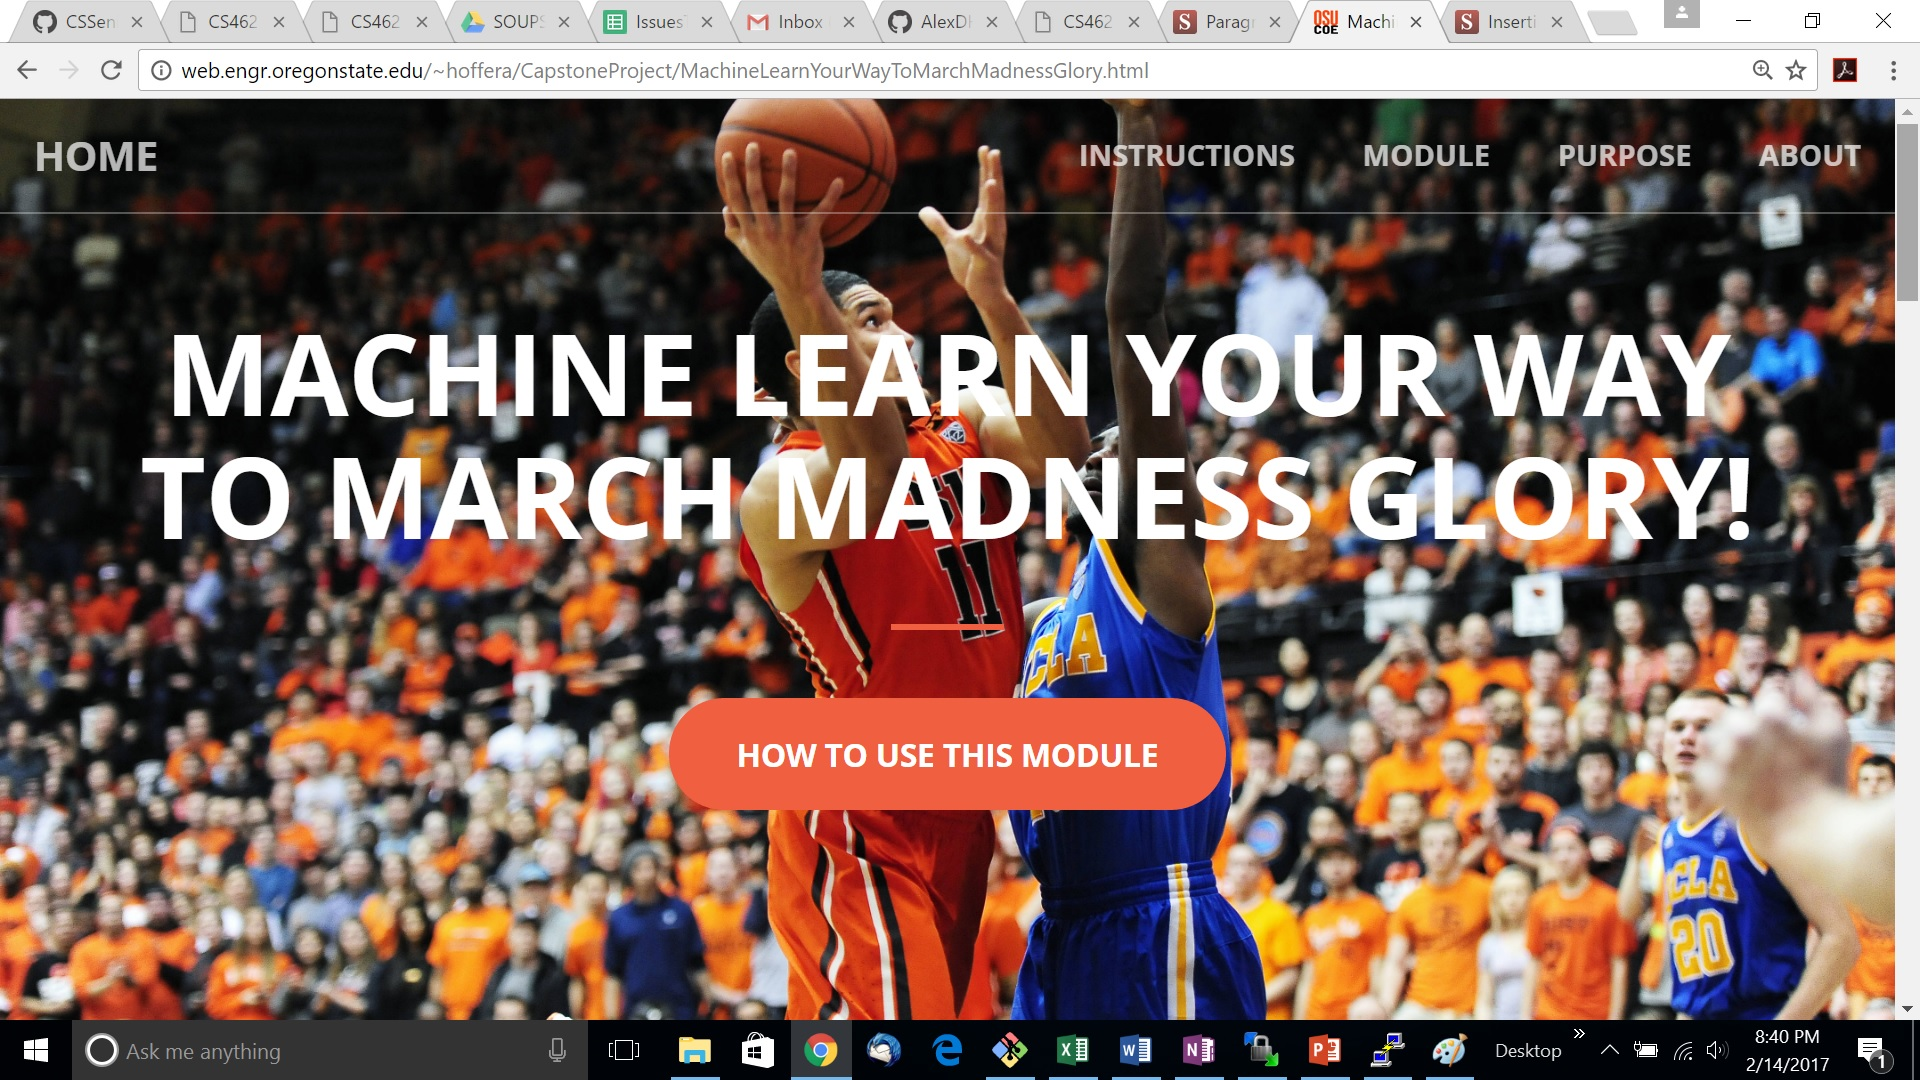
\includegraphics[width=0.8\textwidth]{images/dv}
\caption{A home page where the user can go anywhere in the project using "Menu" or go immediately to the next section by clicking the button.}
\label{fig1}
\end{figure}

\begin{figure}[H]
\centering
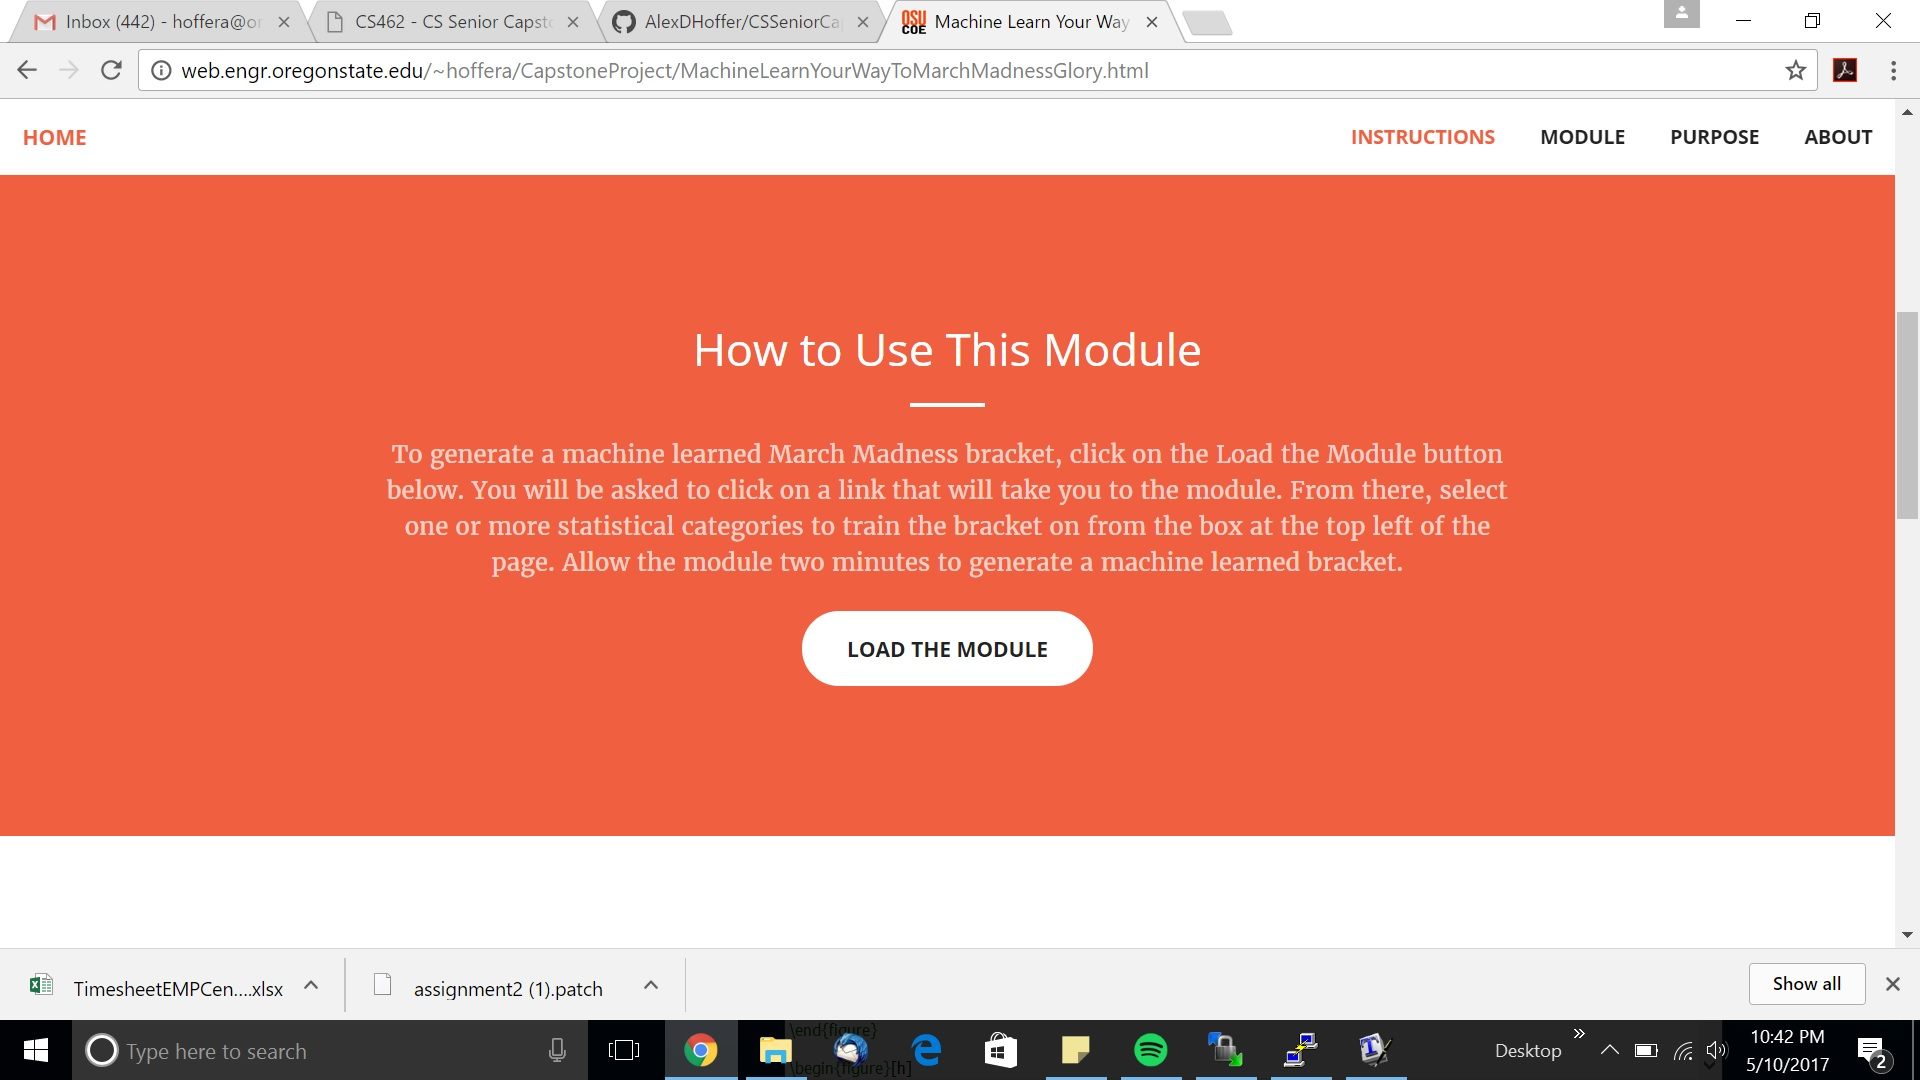
\includegraphics[width=0.8\textwidth]{images/Instructions}
\caption{Instructions on using the module presented before the module itself is presented, as outlined by Responsibility \#2.}
\label{fig2}
\end{figure}

\begin{figure}[H]
\centering
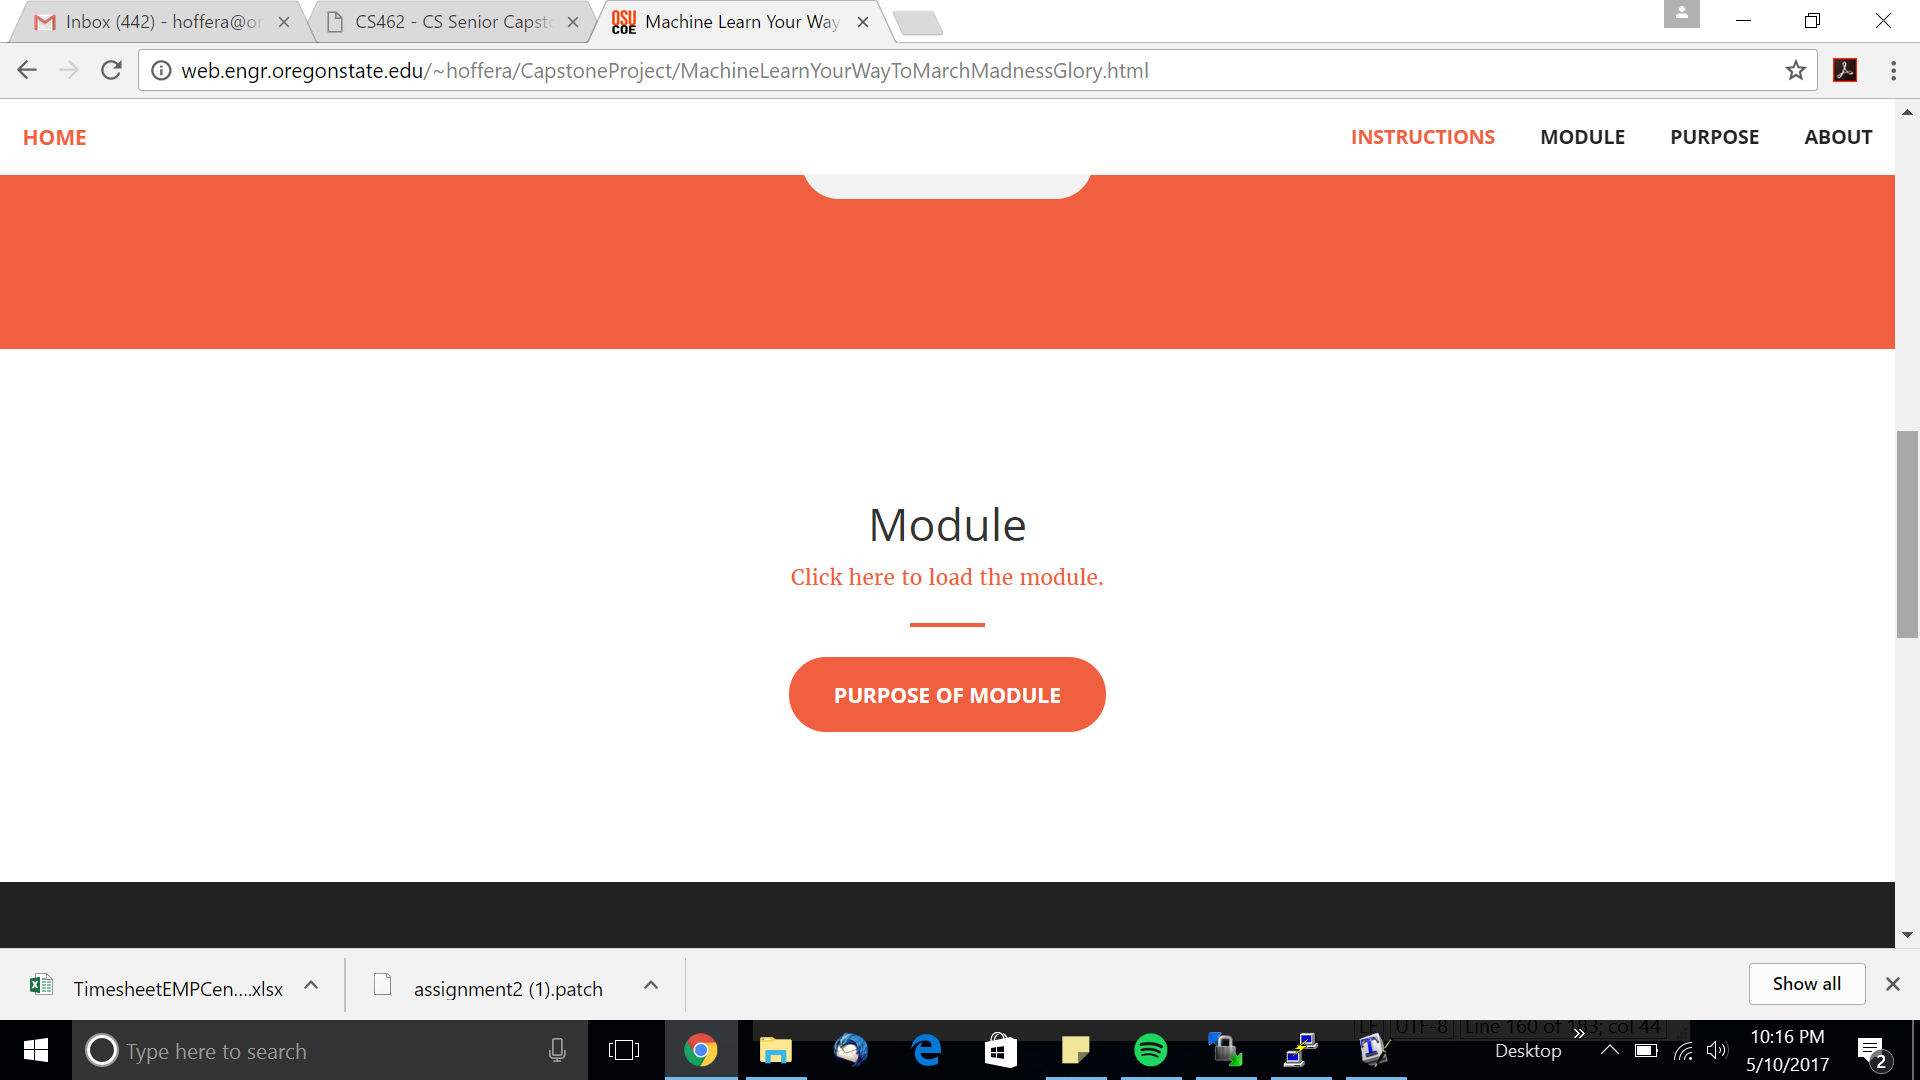
\includegraphics[width=0.8\textwidth]{images/Module}
\caption{A link to the module hosted on AWS.}
\label{fig3}
\end{figure}

\begin{figure}[H]
\centering
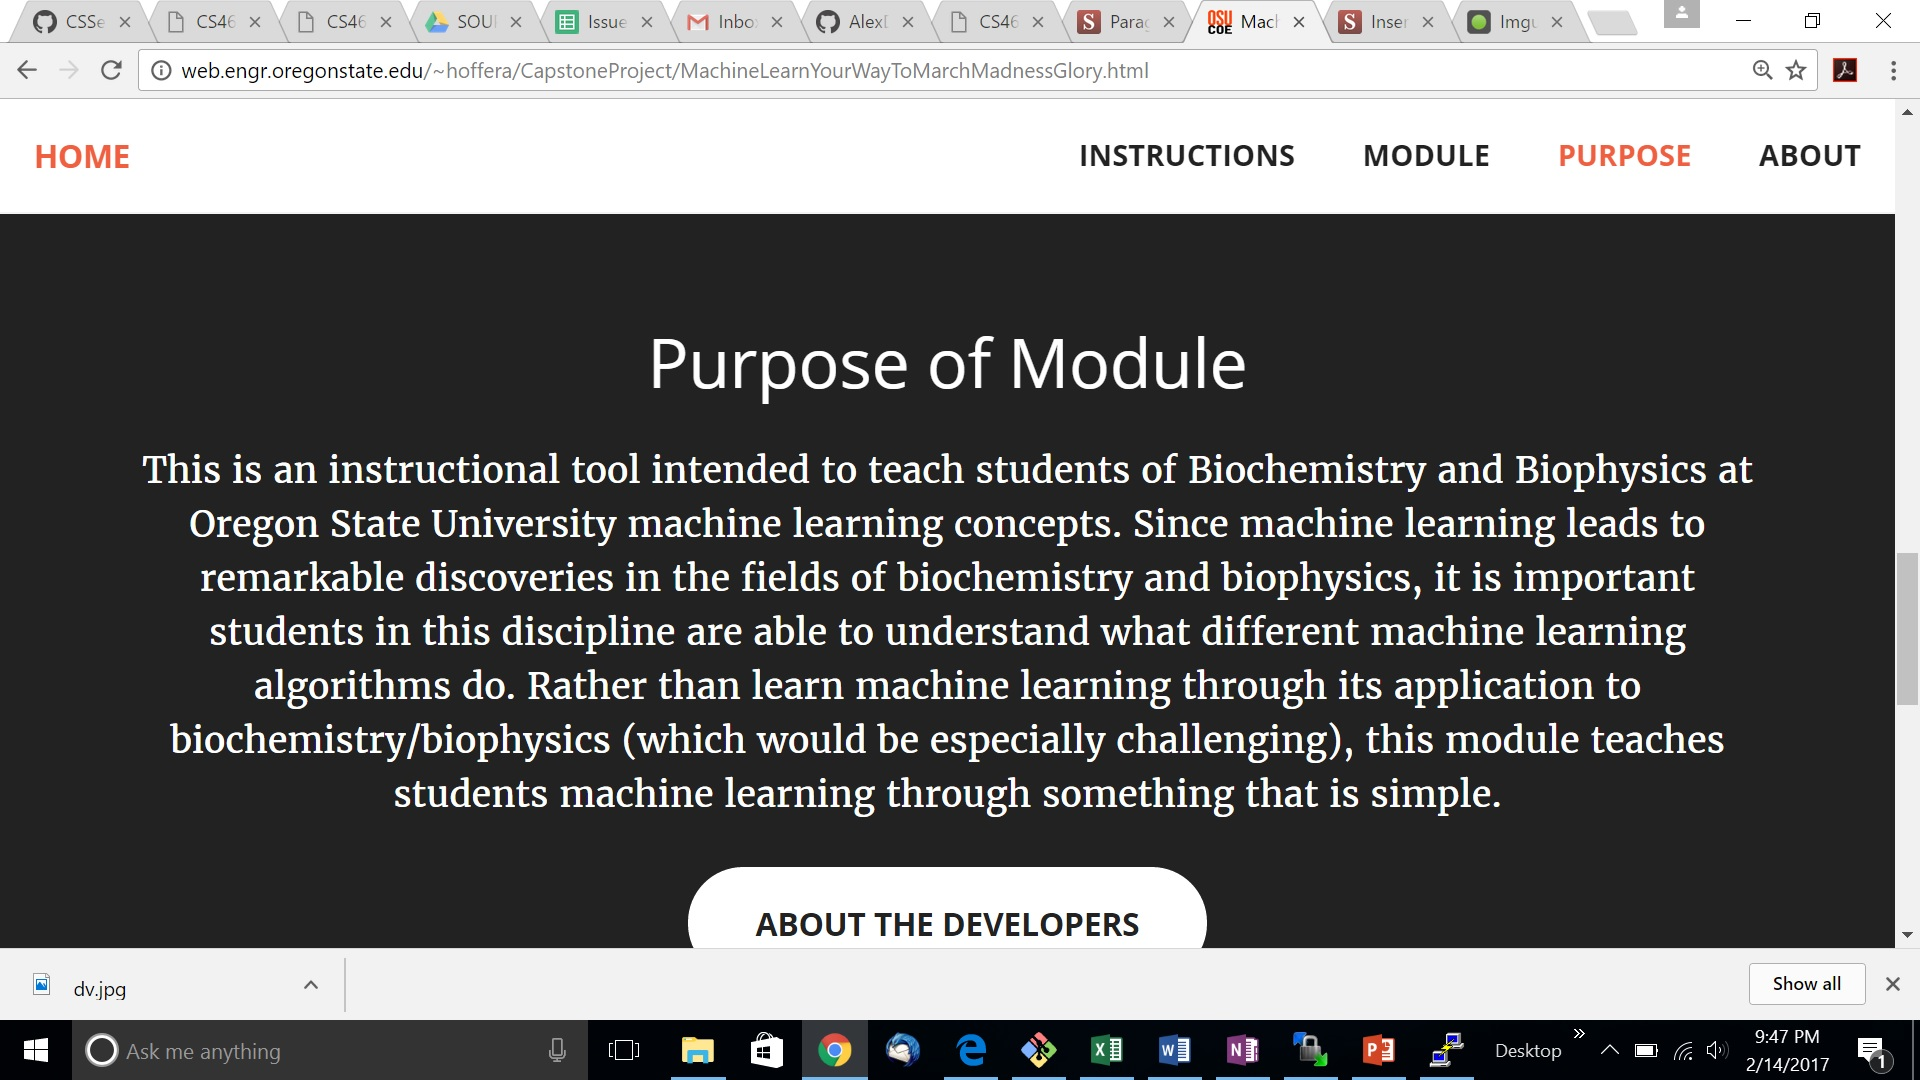
\includegraphics[width=0.8\textwidth]{images/Purpose}
\caption{A page that describes why we did this project.}
\label{fig4}
\end{figure}

\begin{figure}[H]
\centering
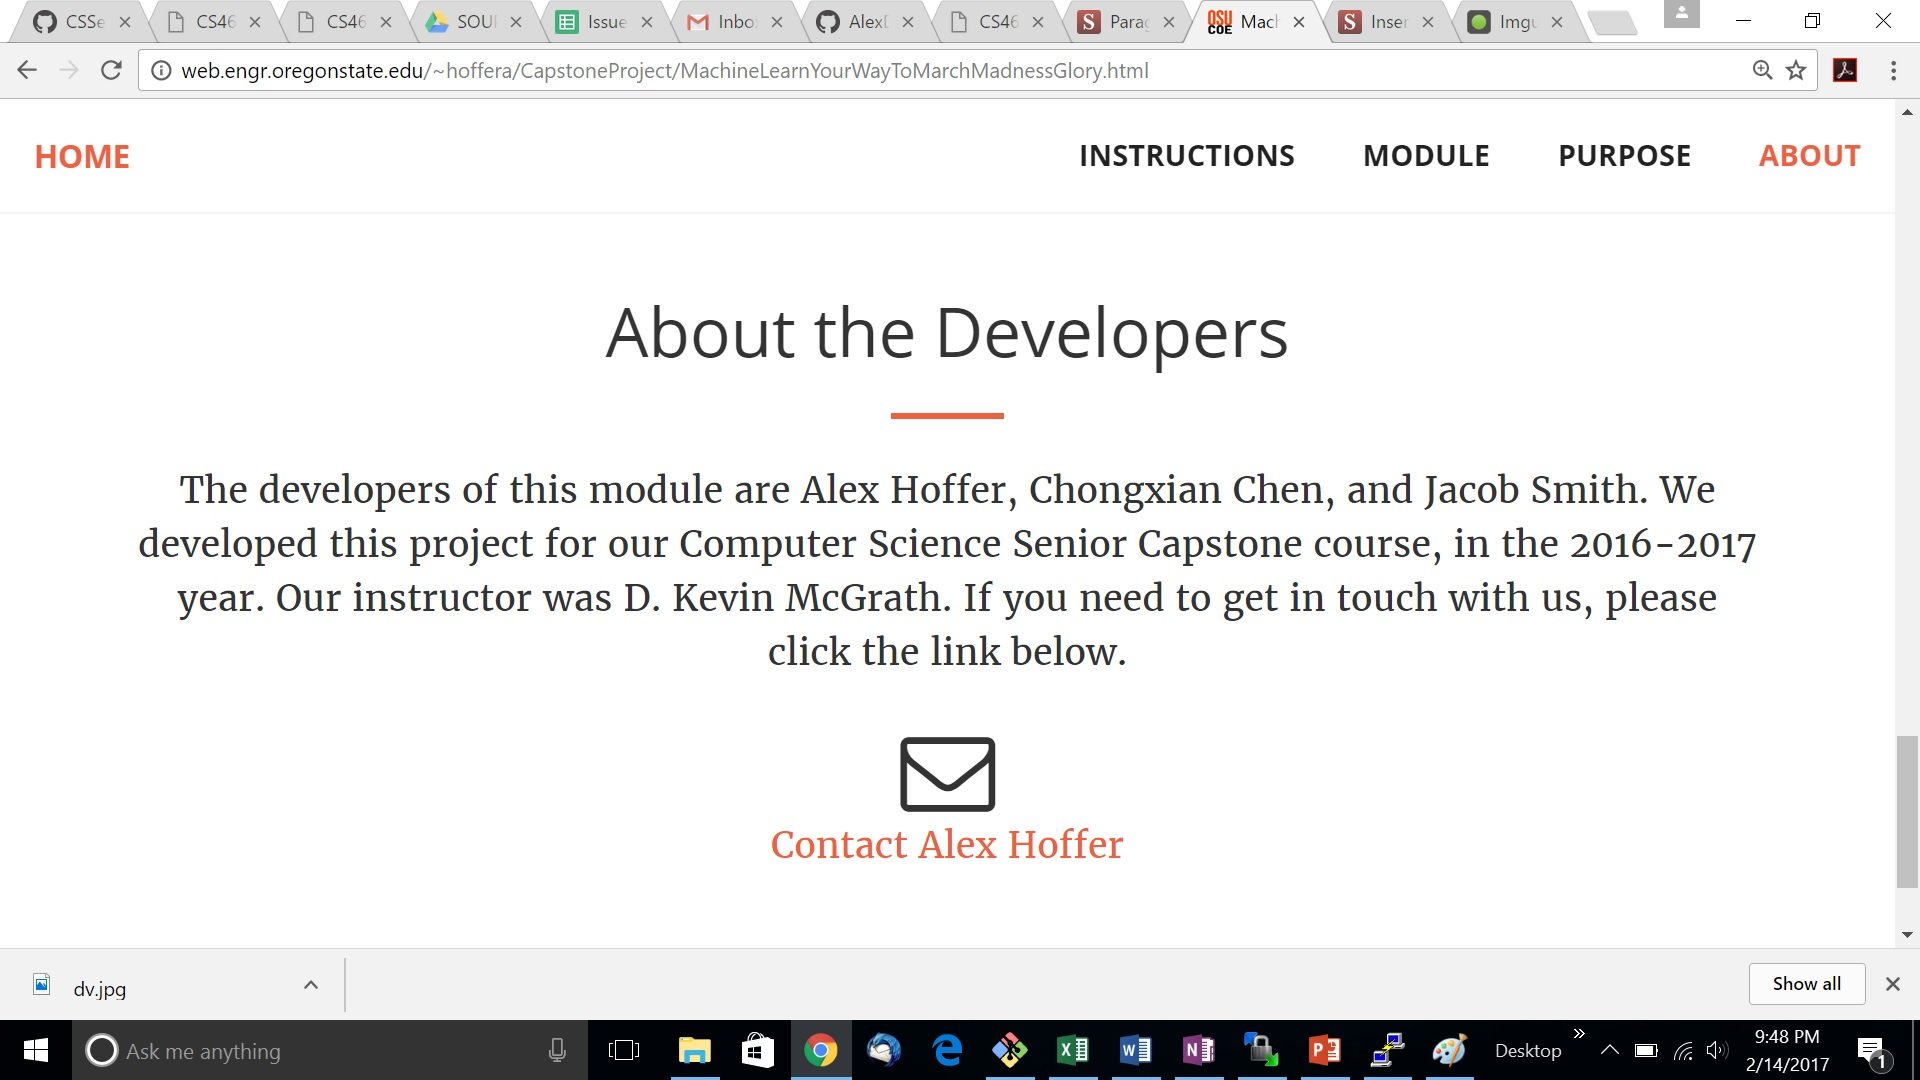
\includegraphics[width=0.8\textwidth]{images/About}
\caption{This page describes who we are and includes a way to contact me.}
\label{fig5}
\end{figure}


\section{Chongxian}
\subsection{Where Chongxian is At On the Project}
Chongxian has completed all functional requirements of the Machine Learning module including different algorithmn and different basketball stats for the users to choose from. The module is also put on Chongxian's Amazon web space so the users are able to run the python module remotely and generate the visible results. 

\subsection{What Chongxian Has Left To Do}
The remaining parts of this class that Chongxian has left to do are: present at Expo, turn in the spring term progress report, and complete the writing assignments needed at the end. Since all the functional requirements are completed, all I can do is to improve the performance even more. The most significant thing I can do is upgrade the Amazon Web Service so users can get their results faster remotely, but that increases the cost. Other things I can do may include introducing more algorithmns to make our module more educational.

\subsection{Problems that have impeded my progress}
At first since none of our team members have taken Machine Learning classes before, I have to explore about it. In the beginning we don't even know what language to use or what library to start with. Our TA Xinze Guan got us started with SciKit Learn library in Python. After spending a long time reseaching, learning and modifying our script, the functional module is completed. During the process I got a lot helps from the website Kaggle.com and Jake. Then we found that OSU server doesn't run Python script. Then I moved to Amazon Web Service (AWS). But the AWS free machine has too small memory so I spend a while figuring out how to install all the required Python environments for our project. 
Visualizing our results also met difficulties on AWS since there is no monitor part on AWS server, it purely is a computing machine. Thus PIL in Python got some trouble. After troubleshooting I finally figure it out and our module is successfully ran on it. 

\subsection{Particularly interesting pieces of code}
\begin{lstlisting}[caption=Python command line arguments that allow users to use different algorithmns from SciKit Learn, label=list2]
if len(sys.argv) > 1:
      if sys.argv[1] == '1':
        print("You choose linear logistic regression to be the model")
        model = linear_model.LogisticRegression()
      elif sys.argv[1] == '2':
        print("You choose svm rbf to be the model")
        model = svm.SVC(gamma=0.001, C=100., probability=True, kernel='rbf')
      elif sys.argv[1] == '3':
        print("You choose svm linear to be the model")
        model = svm.SVC(gamma=0.001, C=100., probability=True, kernel='linear')
      elif sys.argv[1] == '4':
        print("You choose svm poly to be the model")
        model = svm.SVC(gamma=0.001, C=100., probability=True, kernel='poly')
      elif sys.argv[1] == '5':
        print("You choose svm sigmoid to be the model")
        model = svm.SVC(gamma=0.001, C=100., probability=True, kernel='sigmoid')
        elif sys.argv[1] == '6':
            print("You choose Niave Bayes Gaussian to be the model")
            model = GaussianNB()
        elif sys.argv[1] == '7':
            print("You choose Niave Bayes multinomial models to be the model")
            model = MultinomialNB()
\end{lstlisting}

\subsection{Images from my parts of the project}
A more in-depth description of the images I'll be including:

\begin{enumerate}
\item The table in \textit{Fig. 6}. The first selection includes 7 algorithms and the second selection include 10 basketball stats where users can choose multiple to generate their prediction.
\item The terminal output when running the Python Script, found in \textit{Fig. 7}, shows the user the detail when running the script like how many samples are used and model selection score.
\item The visualized bracket in \textit{Fig. 8}, shows users their prediction of March Madness 2017
\end{enumerate}  

\begin{figure}[H]
\centering
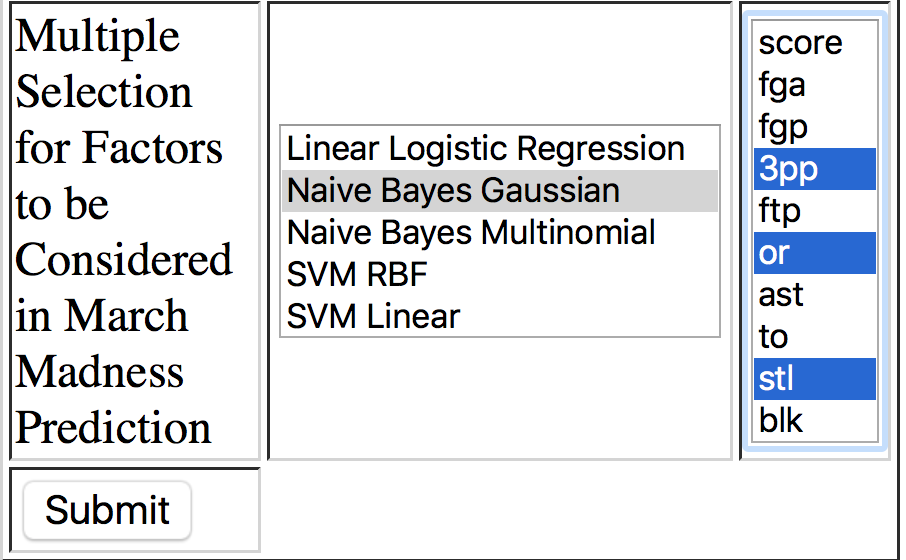
\includegraphics[width=0.8\textwidth]{images/table.png}
\caption{HTML table to allow users to choose algorithmns and stats}
\label{fig6}
\end{figure}

\begin{figure}[H]
\centering
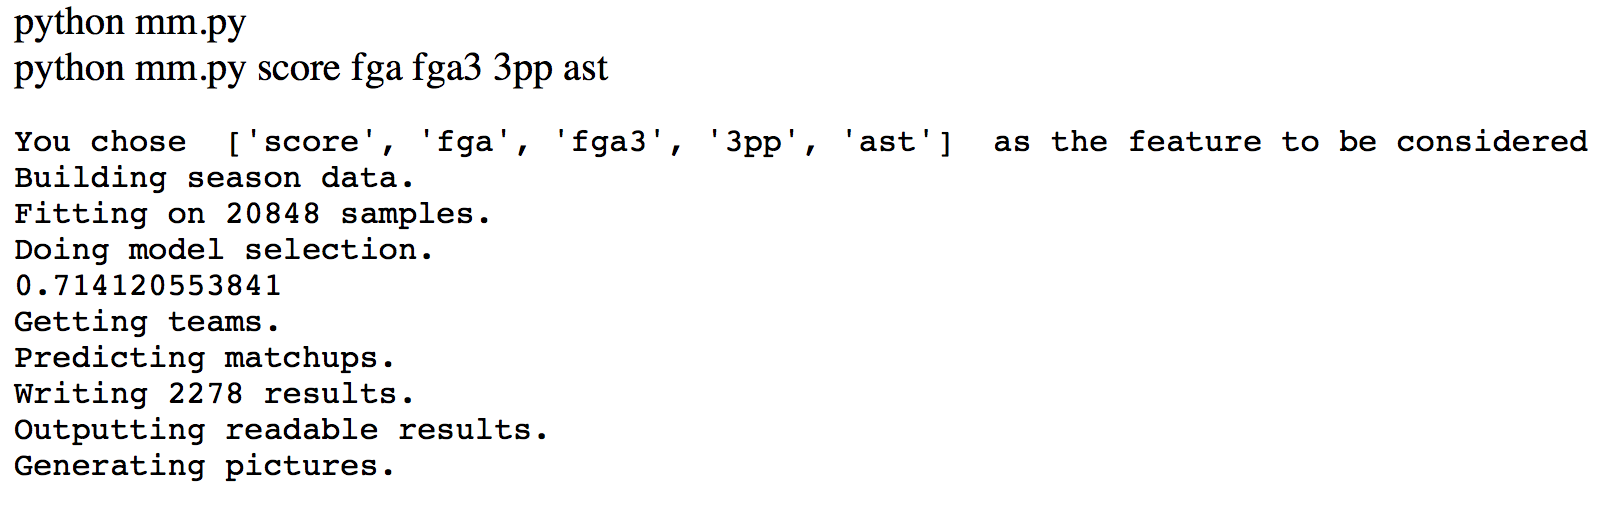
\includegraphics[width=1\textwidth]{images/result.png}
\caption{The terminal output when executing the Puython script}
\label{fig7}
\end{figure}

\begin{figure}[H]
\centering
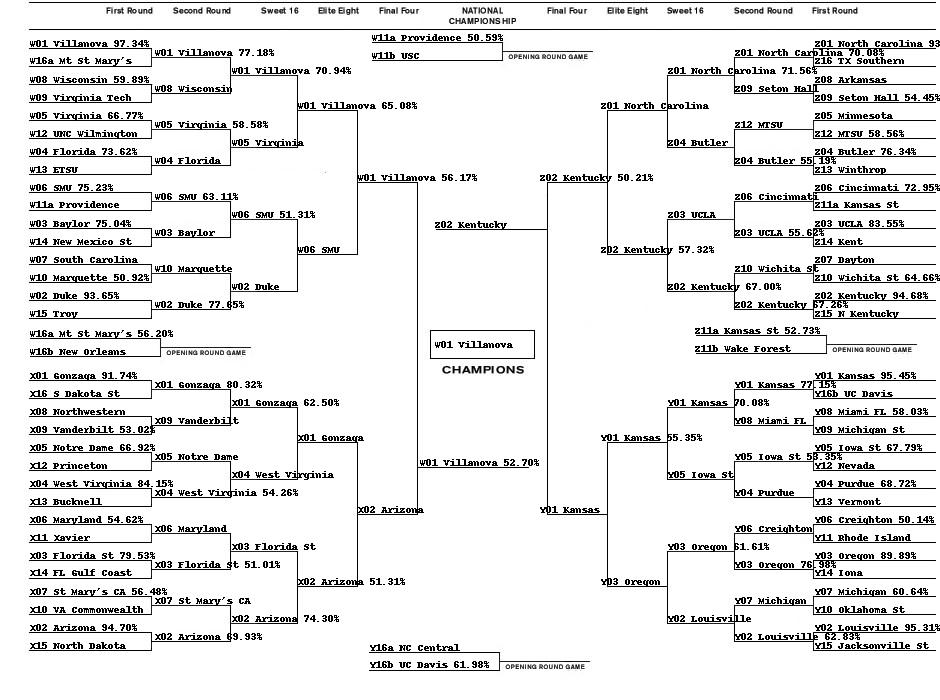
\includegraphics[width=1\textwidth]{images/bracket.jpg}
\caption{Visualization of our final result as a bracket}
\label{fig8}
\end{figure}


\section{Jacob}

\subsection{Where Jake is At On the Project}
Jake completed his requirements at the end of last term once the final regular season game was played for the 2016-2017 Men’s NCAA Basketball season. Since then the only thing I can do is collect additional tournament stats or more in-depth season stats. Either way I would have to introduce those into the algorithms which could cause bugs or throw our predictions off. Because of this we have not added them to our expo module as it currently satisfies all functional requirements.  The additional stats have the possibility to make our module more accurate and therefore more appealing to outside audiences.

\subsection{What Jake Has Left To Do}
The remaining parts of this class Jake has left to do are: The spring report demo, the expo, and complete the remaining writing for the upcoming assignments. In terms of technical parts left that need to be addressed, there are none except for possible future versions if so inclined. All requirements are completed and fully functional.

\subsection{Problems that have impeded my progress}
My first issue was finding a good website to scrap my data from. Some sites had duplicate data or just very confusing navigation through their sites. After that I had issues gathering the data I wanted and cleaning it up to be put in the database. An issue I was stuck on for a while was making sure I didn’t scrape duplicate stats for the same games or teams, which happened a lot more then I hoped. My next issue once I got all the data I needed was to help George with getting the bracket to automatically fill in with the predictions from his algorithms. Another big issue we ran into was hosting the python scripts. At first we tried to host them on our OSU server accounts but were not able to host embedded python scripts because it is a security risk. We had to then host our scripts of Georges AWS account which works great but the free version is a bit slow if given to much data.

\subsection{Particularly interesting pieces of code}
\begin{lstlisting}[caption=Extract the data from the boxscore's url and store in gaame object, label=list3]

                    game_url = 'http://scores.espn.go.com' + url
                    try:
                        gm_info, gm_players, gm_stats = get_data(game_url, ua, tourney_df, ncaa)
                        gen_info.append(gm_info)
                        if gm_players is not None:
                            players.append(gm_players)
                            game_stats.append(gm_stats)
                    except:
                        f = open('Last_Day_Parsed', 'w')
                        f.write(day)
                        f.close()
                        f2 = open('Failed_Game', 'w')
                        box = game_url.split('.com')[-1]
                        f2.write(box)
                        f2.close()
                        print "Broke off loop at ", game_url
                        return gen_info, players, game_stats
\end{lstlisting}

 





\end{document}
